\documentclass[conference]{IEEEtran}
\IEEEoverridecommandlockouts
% The preceding line is only needed to identify funding in the first footnote. If that is unneeded, please comment it out.
\usepackage{cite}
\usepackage{amsmath,amssymb,amsfonts}
\usepackage{algorithmic}
\usepackage{graphicx}
\graphicspath{{../report_figures/}}
\usepackage{textcomp}
\usepackage{xcolor}
\usepackage{url}
\def\BibTeX{{\rm B\kern-.05em{\sc i\kern-.025em b}\kern-.08em
    T\kern-.1667em\lower.7ex\hbox{E}\kern-.125emX}}
\begin{document}

% NOTE (IEEE rule): no symbols, special characters, footnotes, or math in the title.
\title{How Time Flies: Emotional and Sonic Change in Music, 1990--2022}

\author{\IEEEauthorblockN{Yürekçe Altın}
\IEEEauthorblockA{\textit{Computer Engineering} \\
\textit{Middle East Technical University}\\
Ankara, Türkiye \\
yurekce.altin@metu.edu.tr}
}

\maketitle

\begin{abstract}
    How has the produced music changed over the last three decades? 
    We analyze the emotional and sonic change in produced music from 
    1990 to 2022 using a dataset from Spotify which includes 489.761 
    songs, their lyrics and sonic features. A Spark pipeline and BERT 
    lyrics-emotion classification, K-Means valence and energy era 
    discovery, and Mann-Kendall change point testing has been made. 
    Over 33 years, we find that from 1990 to 2022, valence (22\%) , 
    acousticness (29\%), and duration (decreased), while energy (18\%), 
    tempo (+4.9BPM), and loudness (+3.7 dB) have increased. 
    The lyrics contains less words about love and more words 
    about loneliness. The dominant turning point is around 2000, 
    which is consistent across all methods.
\end{abstract}

\begin{IEEEkeywords}
music information retrieval, emotion classification, BERT, Apache Spark, trend analysis, change-point detection
\end{IEEEkeywords}

\section{Introduction}

We humans evolve with time and what it brings. Music has been a way for humans to express themselves. This study aims to look at the change of sonic feautures and lyric emotions in the music spanned over the years. Previous studies on this mostly used context-blind lexicons or small datasets. We aim to use a BERT emotion model on the lyrics of 489.761 songs from 1990 to 2022, which extracts the probability of the lyrics' dominant emotion out of love, joy, anger, sadness and fear. We also analyze the audio features of the songs, including valence, energy, loudness, acousticness, tempo and duration. We then analyze the trends of these features over time and detect change points in the data. We also use K-Means clustering to discover eras in the music based on valence and energy.
% Motivation: do popular songs get sadder / less loving over three decades?

\subsection{Problem Statement}
We ask whether the emotional and sonic character of popular music changed
measurably between 1990 and 2022:

\begin{itemize}
  \item \textbf{RQ1.} Do lyric emotions show significant patterns over time?
  \item \textbf{RQ2.} Do audio features (valence, energy, loudness, tempo,
        \dots) show significant trends?
  \item \textbf{RQ3.} Does valence and energy clustering reveal discrete eras?
\end{itemize}


\subsection{Contributions}
\begin{itemize}
  \item \textbf{Mood and lyric emotion at scale.} Sound (ten audio features) and
        words (BERT lyric emotion) measured across 489{,}761 songs over
        three decades.
  \item \textbf{Validated with statistics.} Mann--Kendall, Sen's slope,
        Benjamini--Hochberg FDR, change-point detection, and Pettitt's test
        implemented from scratch and cross-checked against SciPy, statsmodels,
        and ruptures---every figure auditable.
  \item \textbf{Comparing results for yearly differences.} Break years from all analyses
        synthesized into one timeline, converging on a dominant turning point
        around the year 2000.
\end{itemize}

\section{Dataset}
\label{sec:dataset}

\subsection{Source and Scope}
Our data is the public ``550K+ Spotify Songs (Audio, Lyrics, and Genres)''
dataset \cite{b_dataset}, distributed as two CSV exports named artists.csv and songs.csv, 
which we used the later one directly. Each record pairs a track's Spotify audio features with its full
lyrics, fetched from LRCLIB, and a main genre mapped to one of ten standard
categories. For each song the dataset provides ten numeric audio descriptors
(danceability, energy, loudness, speechiness, acousticness, instrumentalness,
liveness, valence, tempo, and duration), the lyrics, the release year, genre and
sub-genres, popularity, and artist metadata. We analyze all ten audio features
together with the lyrics, which carry our two complementary views of mood:
how a song \emph{sounds} and what it \emph{says}.

We restricted our data from 1990 through 2022 because the sample size was too small 
to make a healthy analysis before 1990 and after 2022.
\textbf{489{,}761} songs is what we were left with. Coverage
is still uneven across the window: the catalog grows by roughly an order of magnitude
over the three decades, a property we account for explicitly in
Section~\ref{sec:methodology} to ensure the observed trends reflect musical change rather
than corpus growth.
% Spotify dataset [cite], 1990--2022; number of songs and lyrics; per-year counts.

\subsection{Cleaning and Filtering}
\texttt{songs.csv} is read with Spark in multiline mode, with
quote and escape handling enabled so that the commas and line breaks embedded in
lyrics are parsed correctly rather than splitting records. Then we apply our three
cleaning steps. We first filter out songs with a release year outside of 1990 and 2022,
then we filter out the ones with an invalid valence, which is below zero or above one,
and lastly, we remove songs without lyrics, genre, year, track identifier, popularity, or
sub-genre. The lyrics is normalized in two different ways for two different tasks.
For the love, lust and loneliness lexicon-based analysis, we flatten the lyrics
to a single white-space normalized string. For BERT analysis, it is important to fit
into the token limit, process efficiently, and preserve the meaning.
So for BERT, we preserve the line breaks and split the lyrics into eight-line chunks, 
which are then de-duplicated before ingress.
% Year and valence bounds, null handling.

\section{Methodology}

\subsection{System Architecture and the Spark Pipeline}
The analysis is made as a single Apache Spark job that runs locally on
all available cores (\texttt{local[*]}). The pipeline works in five stages:
(i) load the raw export; (ii) clean it (Section~\ref{sec:dataset});
(iii) aggregate each audio feature by year; (iv) cluster years into eras; and
(v) classify lyric emotion with BERT and persist a dominant emotion per song.
The cleaned data frame is reused by every analyzer, so it is cached with the
\texttt{MEMORY\_AND\_DISK} storage level once, right after filtering.

BERT analysis is expensive, to fasten it we found two solutions. First, 
lyric chunks are de-duplicated before ingress, yet the count of how many times
it has been repeated is kept, so the emotional data is not lost.
Second, output is \emph{checkpointed per year}: each year is written to its
own partition with a \texttt{\_SUCCESS} marker, so if a job fails, or is interrupted
for any reason, it can continue where it has left of without losing progress.

\subsection{Audio-Feature Aggregation}
For each of the ten audio features we compute its mean over all songs
released in a given year, outputting a 33 year time series of features.

\subsection{Lyric Emotion Classification with BERT}
Lyric emotion is made with the \texttt{bert\_sequence\_classifier\_emotion}
model from Spark NLP~\cite{b_sparknlp}, a BERT sequence classifier~\cite{b_bert} fine-tuned to
five classes: joy, sadness, anger, love, and fear~\cite{b_emotion}. Due to 
lyric being long and exceeding the token limit of the mdoel, we separate each song's lyrics
into eight-line \emph{chunks}. BERT classifier model has a maximum sentence length of 
128 tokens and a batch size of 32. Every chunk gets labeled by one of the 
five emotions based on their highest probability, and after every chunk's
highest probability emotion is found and added up with other chunks' emotion counts $c_e$ for
$e \in \{\text{joy, sadness, anger, love, fear}\}$, the song's dominant emotion is 
determined by the highest count, $\hat{e} = \arg\max_e c_e$. To ensure ties are broken
fairly, when $k$ emotions share the highest count we do not award the whole song to a
single emotion; instead each tied emotion receives an equal vote of $1/k$. Every song
therefore contributes a total weight of exactly one to its year, so the yearly emotion
shares still sum to one while no emotion is favored by an arbitrary ordering.

\subsection{Lexicon-Based Theme Detection}
We also were curious about how the frequency of the words we associated with
 love, lust and loneliness changed over the years. we created three categories 
 of words for each and counted their occurances in lyrics of every song, and added
 up by year and divided the number by how many songs were released that year.

\subsection{K-Means}
A question arose in our minds: if humans were reporting more anxious feelings
and dissatisfaction with their lives, was music a reflection of that? For
answers, we did a K-Means clustering to see how years grouped together based
on their valence and energy axes. Each dimension is standardized to zero mean and unit
variance before clustering so that features on different scales contribute
equally. The number of clusters isn't fixed, we run K-Means for
$K = 2,\dots,10$, record the within-set sum of squared errors (WSSSE) for each,
and select the elbow automatically with the Kneedle heuristic~\cite{b_kneedle}.

\subsection{Statistical Analysis}
For every type of analysis, results are a time series of 33 years. Our concern
is whether the analysis of audio features or BERT emotions analysis shows
a trend and is there a particular year where multiple features shift.

\subsubsection{Trend Testing}
We use Mann-Kendall test, a standard non-parametric trend test. It uses
every pair of years and counts how often the next year has the higher value.
The result is summarized by Kendall's $\tau$, a number between $-1$ and $+1$ 
($-1$ = always falling, $+1$ = always rising, $0$ = no trend), 
together with a $p$-value for significance. We measure the \emph{size} of a 
trend with Sen's slope, the median yearly change across all pairs of years, 
which is robust to outliers. We control the false-discovery rate with the 
Benjamini--Hochberg correction and report a trend as significant only 
if it survives this stricter bar ($\alpha = 0.05$).

\subsubsection{Change-Point Detection}
We look for sharp turns in the time series. For this, we applied BIC-based
method identifiying the optimal number of change points. We also applied Pettitt's
test to find the most important change point in the series.

\section{Results}

\subsection{Audio-Feature Trends}
Within the ten audio features, five show statistically 
meaniningful results after Benjamini-Hochberg correction at 
$\alpha = 0.05$ (Table~\ref{tab:trends}, Fig.~\ref{fig:tau}).
Strongest decline we see is in valence (Kendall's $\tau = -0.82$, $p < 10^{-9}$), 
which falls by about 22\% compared to its beginning, 1990, level.
Acousticness follows valence by a 29\% decline. We see increases in loudness
by roughly 3.7\,dB, energy by about 18\%, and tempo by about 4.9\,beats per minute.
The music over 33 years seems to have become louder, less acoustic, more energetic,
faster, yet significantly less positive. Also, there seems to be a steady
decrease in duration with a Pettitt change point in 2016.

\subsection{Lyric-Emotion Trends Over Time}
In our analysis it seems to be that joy is the dominant emotion
throughout the years, showing no significant trend. However, the other
four emotions all do. 
Love goes from 3.3\% in 1990 to 2.2\% in 2022, anger falls from 21.1\% to 18.1\%,
sadness rises from 21.1\% to 23.4\%, and fear rises from 2.3\% to 2.5\%.
Four of the five emotions are significant after FDR correction.

\subsection{Lyric Themes: Love, Lust, and Loneliness}
For every category, we have a list of words we look for, case insensitively.
The \emph{love} list is \{heart, love, loved, loving, honey,
stay, angel, trust, promise, forever, miracle, darling, beautiful, cute\}; the
\emph{lust} list is \{body, bodies, kiss, kissing, kissed, touch, touching,
touched, lip, lips, pussy, taste, tasted, tasting, fuck, fucked, fucking\}; and
the \emph{loneliness} list is \{lonely, loneliness, alone, cold, nobody, empty,
silence, silent, lost, numb, isolated\}. For each song we count how many words
fall in each list, then average these counts for each year.

This analysis seems to complement the BERT love results. The density of love 
per song is U-shaped: high in the early 1990s (about 2.9 love words per song),
falling in the mid-2000s (about 2.4), and recovering to its peak by 2022 (about 3.2).
The Pettitt analysis shows us that the year 2000 was the single breaking point.
Lust seems to have 2013 as its breaking point by the Pettitt analysis, and loneliness's
is 2010, increasing after it.

\subsection{Discovered Eras: Mood and Genre Clusters}
We used Kneedle heuristic to select $K = 5$ clusters for valence and energy clustering.
the clusters fall into contiguous bands of years
(Fig.~\ref{fig:mood}): an early- to mid-1990s group, a distinct 2000--2006 band,
a 2007--2011 band, and a long 2012-onward band, with 2022 drifting back toward an
earlier-style cluster. There seems to be a steady fall in valence and a rise in
energy that peaks in the late 2000s and 2010.

% ---- Example figure/table environments wired to your actual outputs. ----
% Single-column figure:
\begin{figure}[htbp]
\centerline{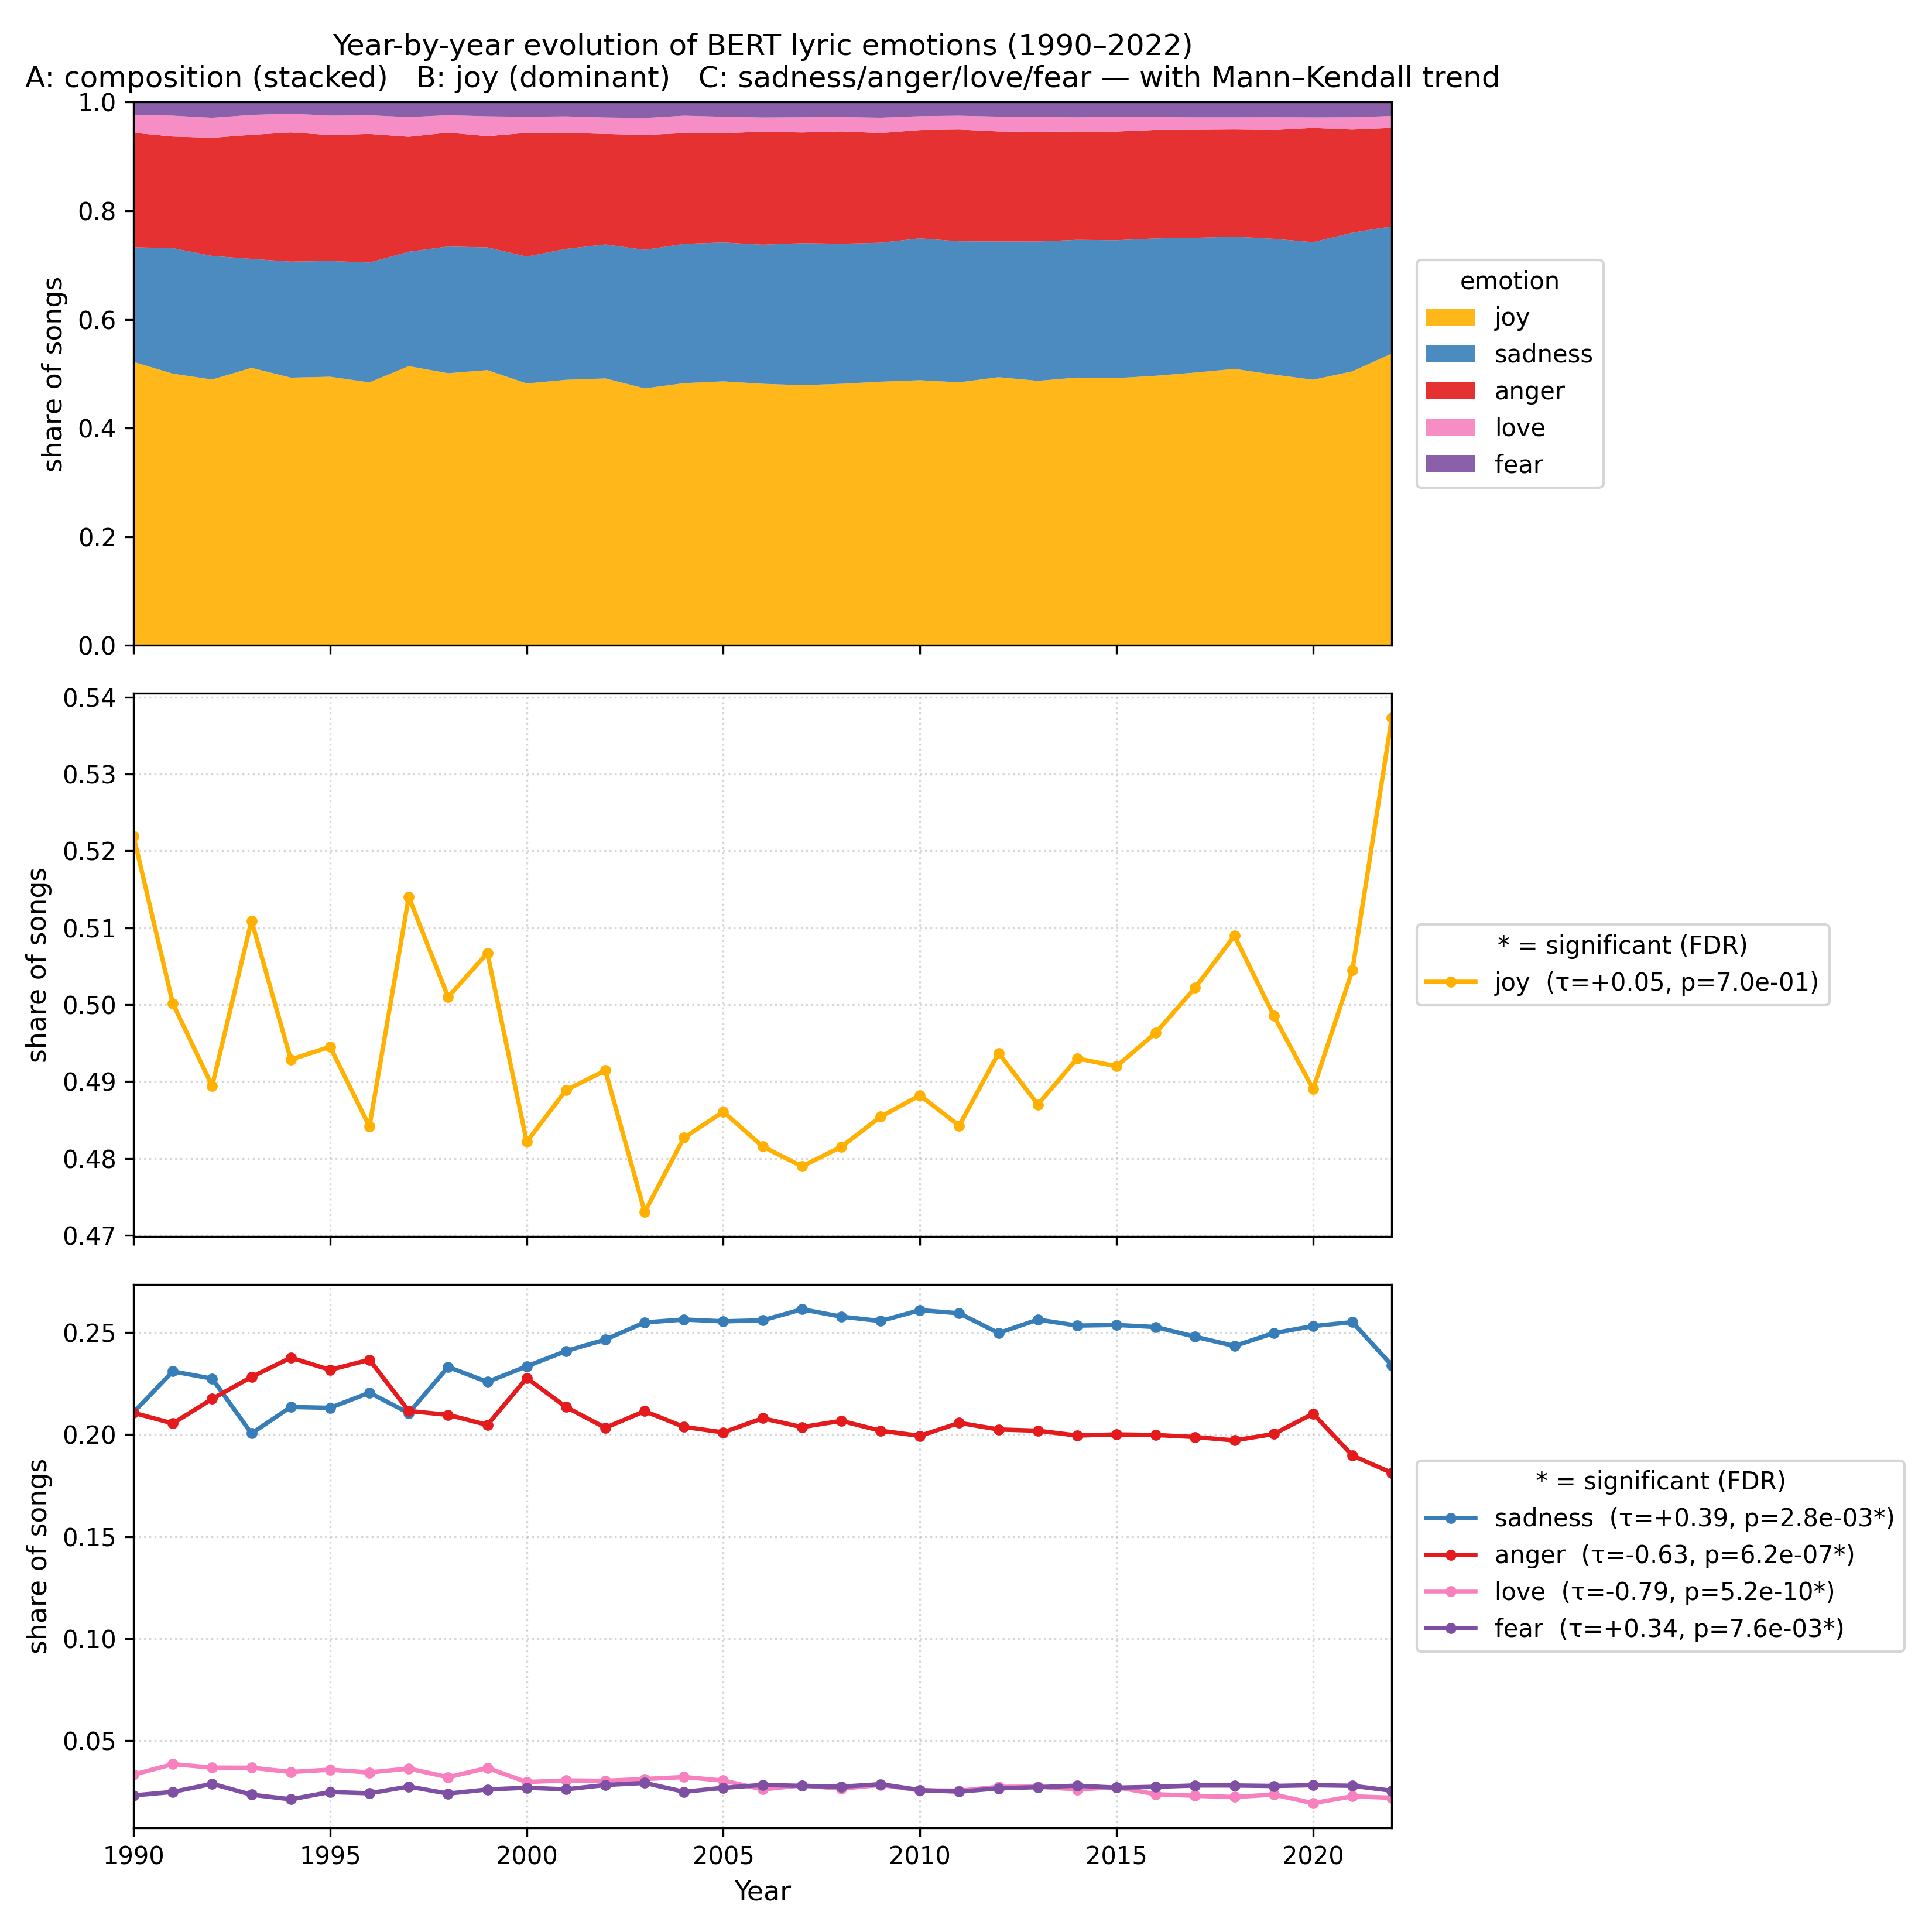
\includegraphics[width=\columnwidth]{fig8_emotion_trends.png}}
\caption{Year-by-year evolution of the five BERT lyric emotions, 1990--2022.}
\label{fig:emotions}
\end{figure}

\begin{figure}[htbp]
\centerline{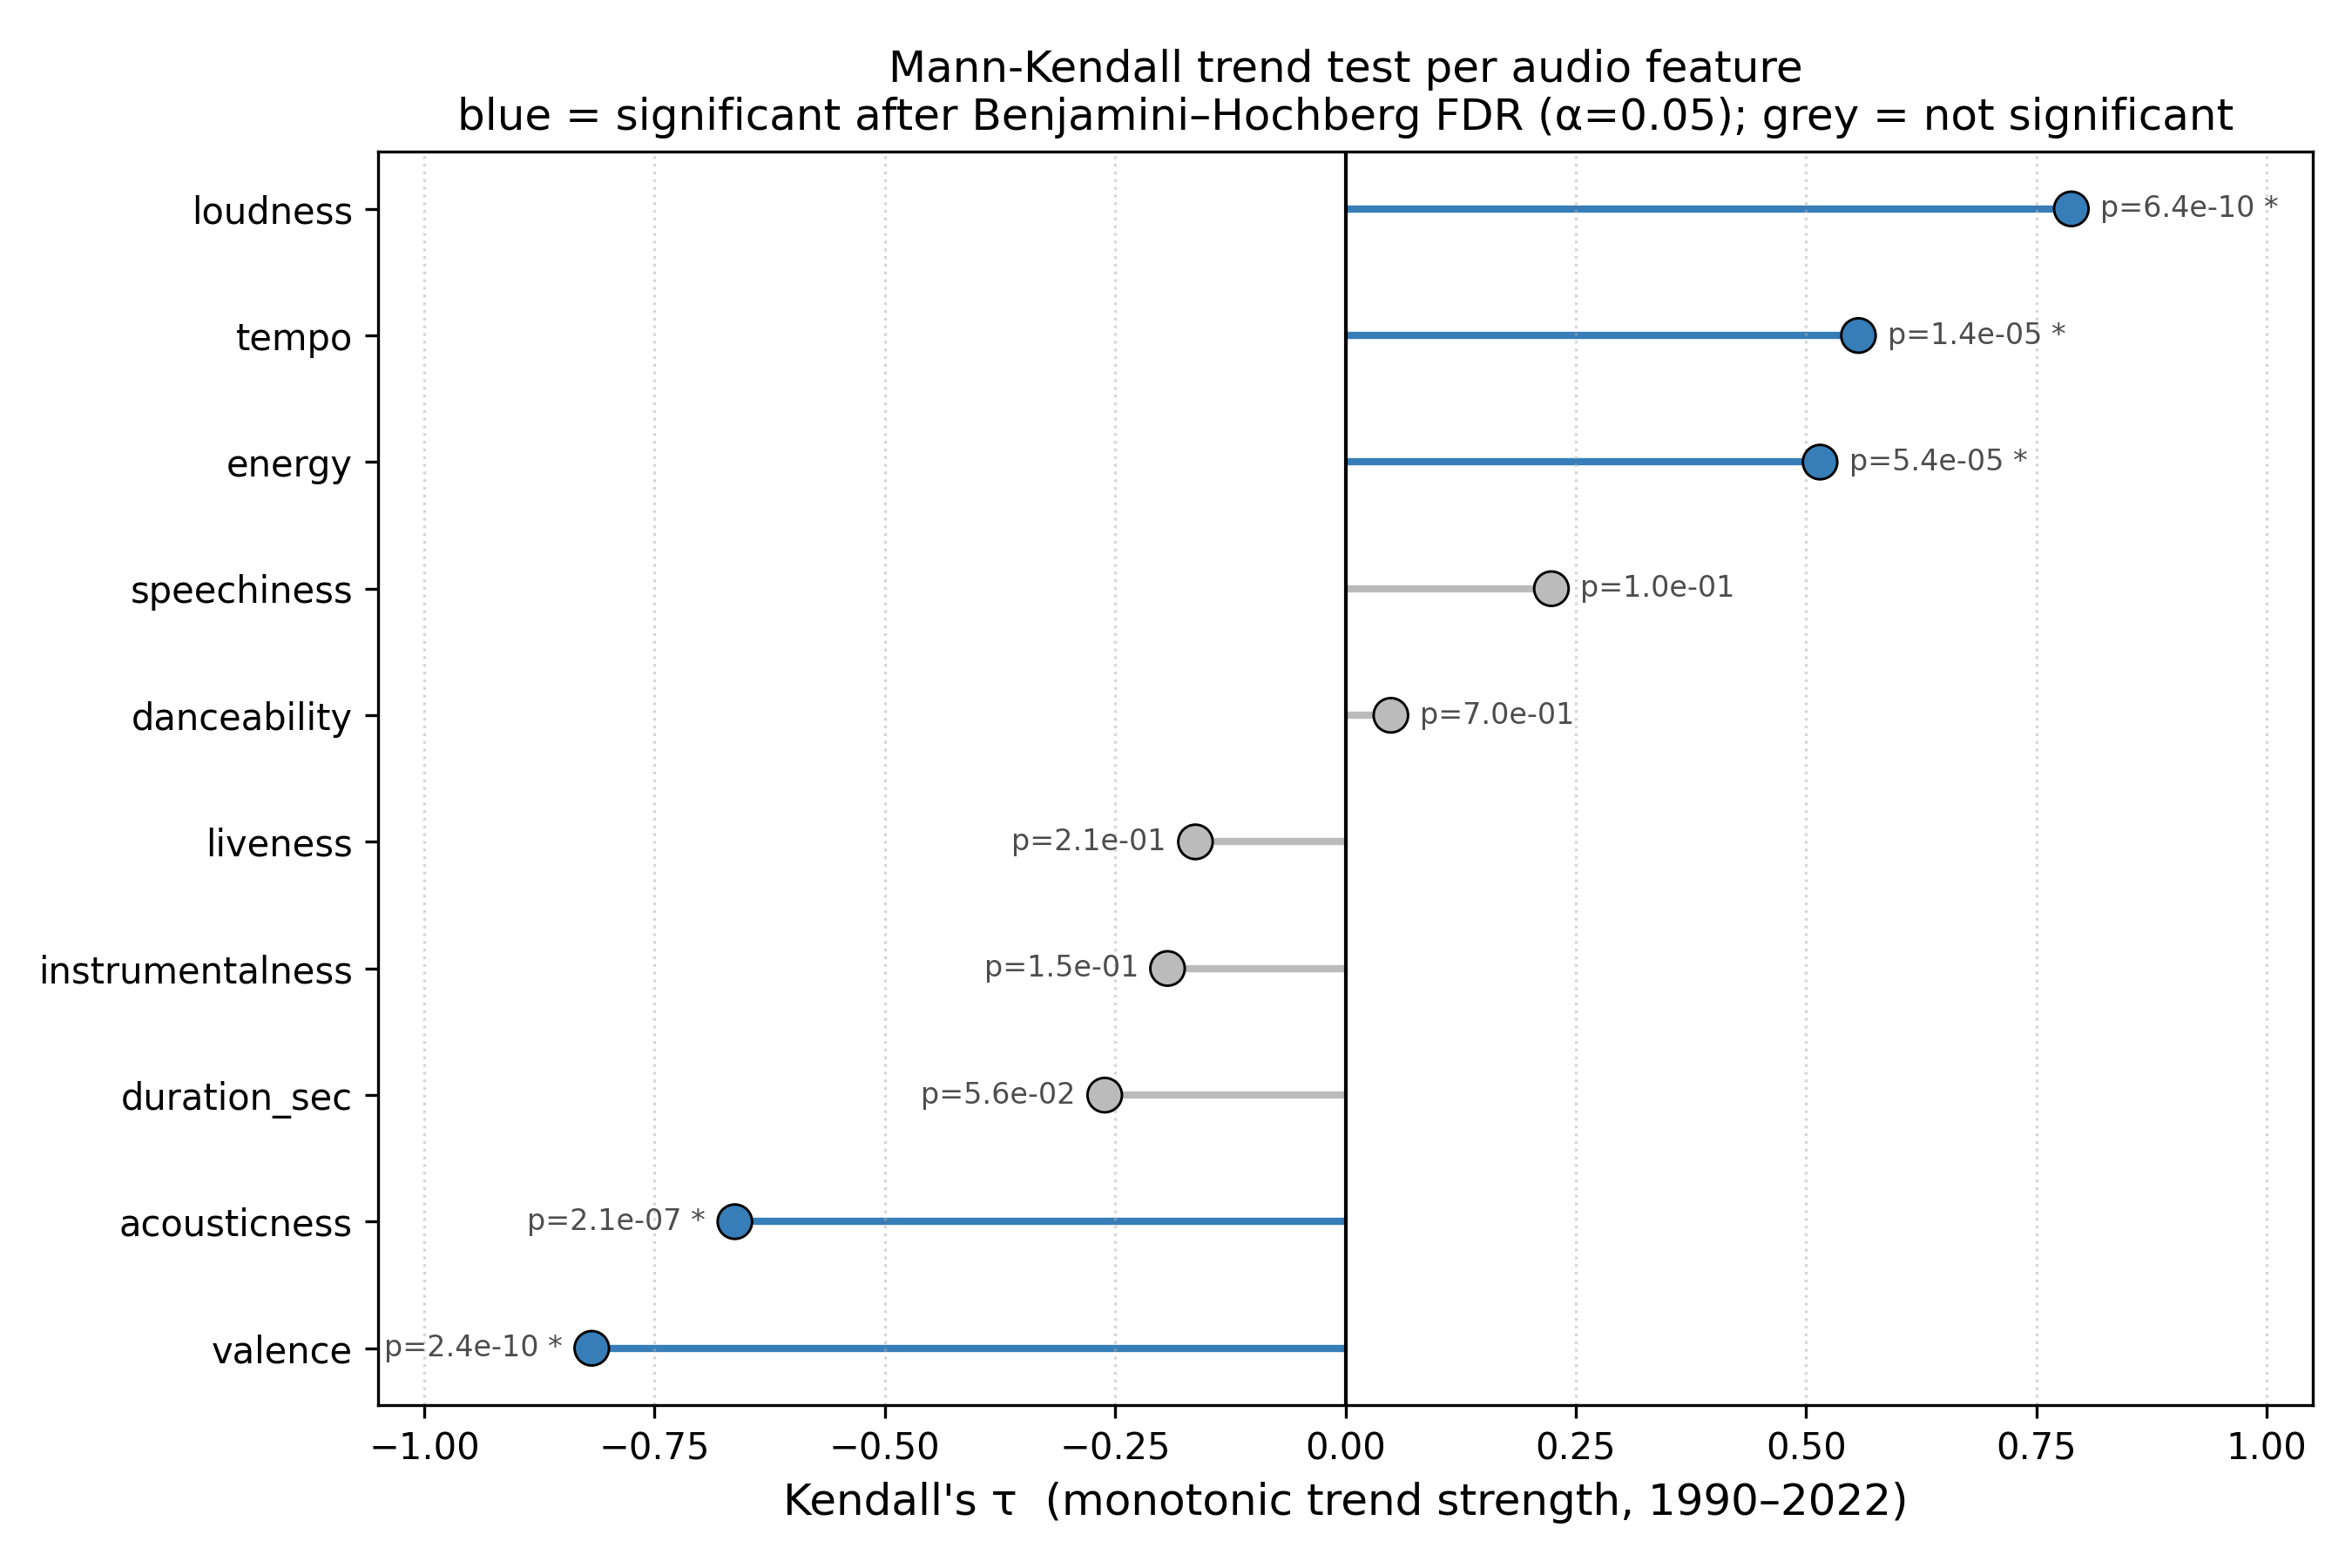
\includegraphics[width=\columnwidth]{fig5_feature_trend_tests.png}}
\caption{Mann--Kendall trend strength per audio feature.}
\label{fig:tau}
\end{figure}

\begin{figure}[htbp]
\centerline{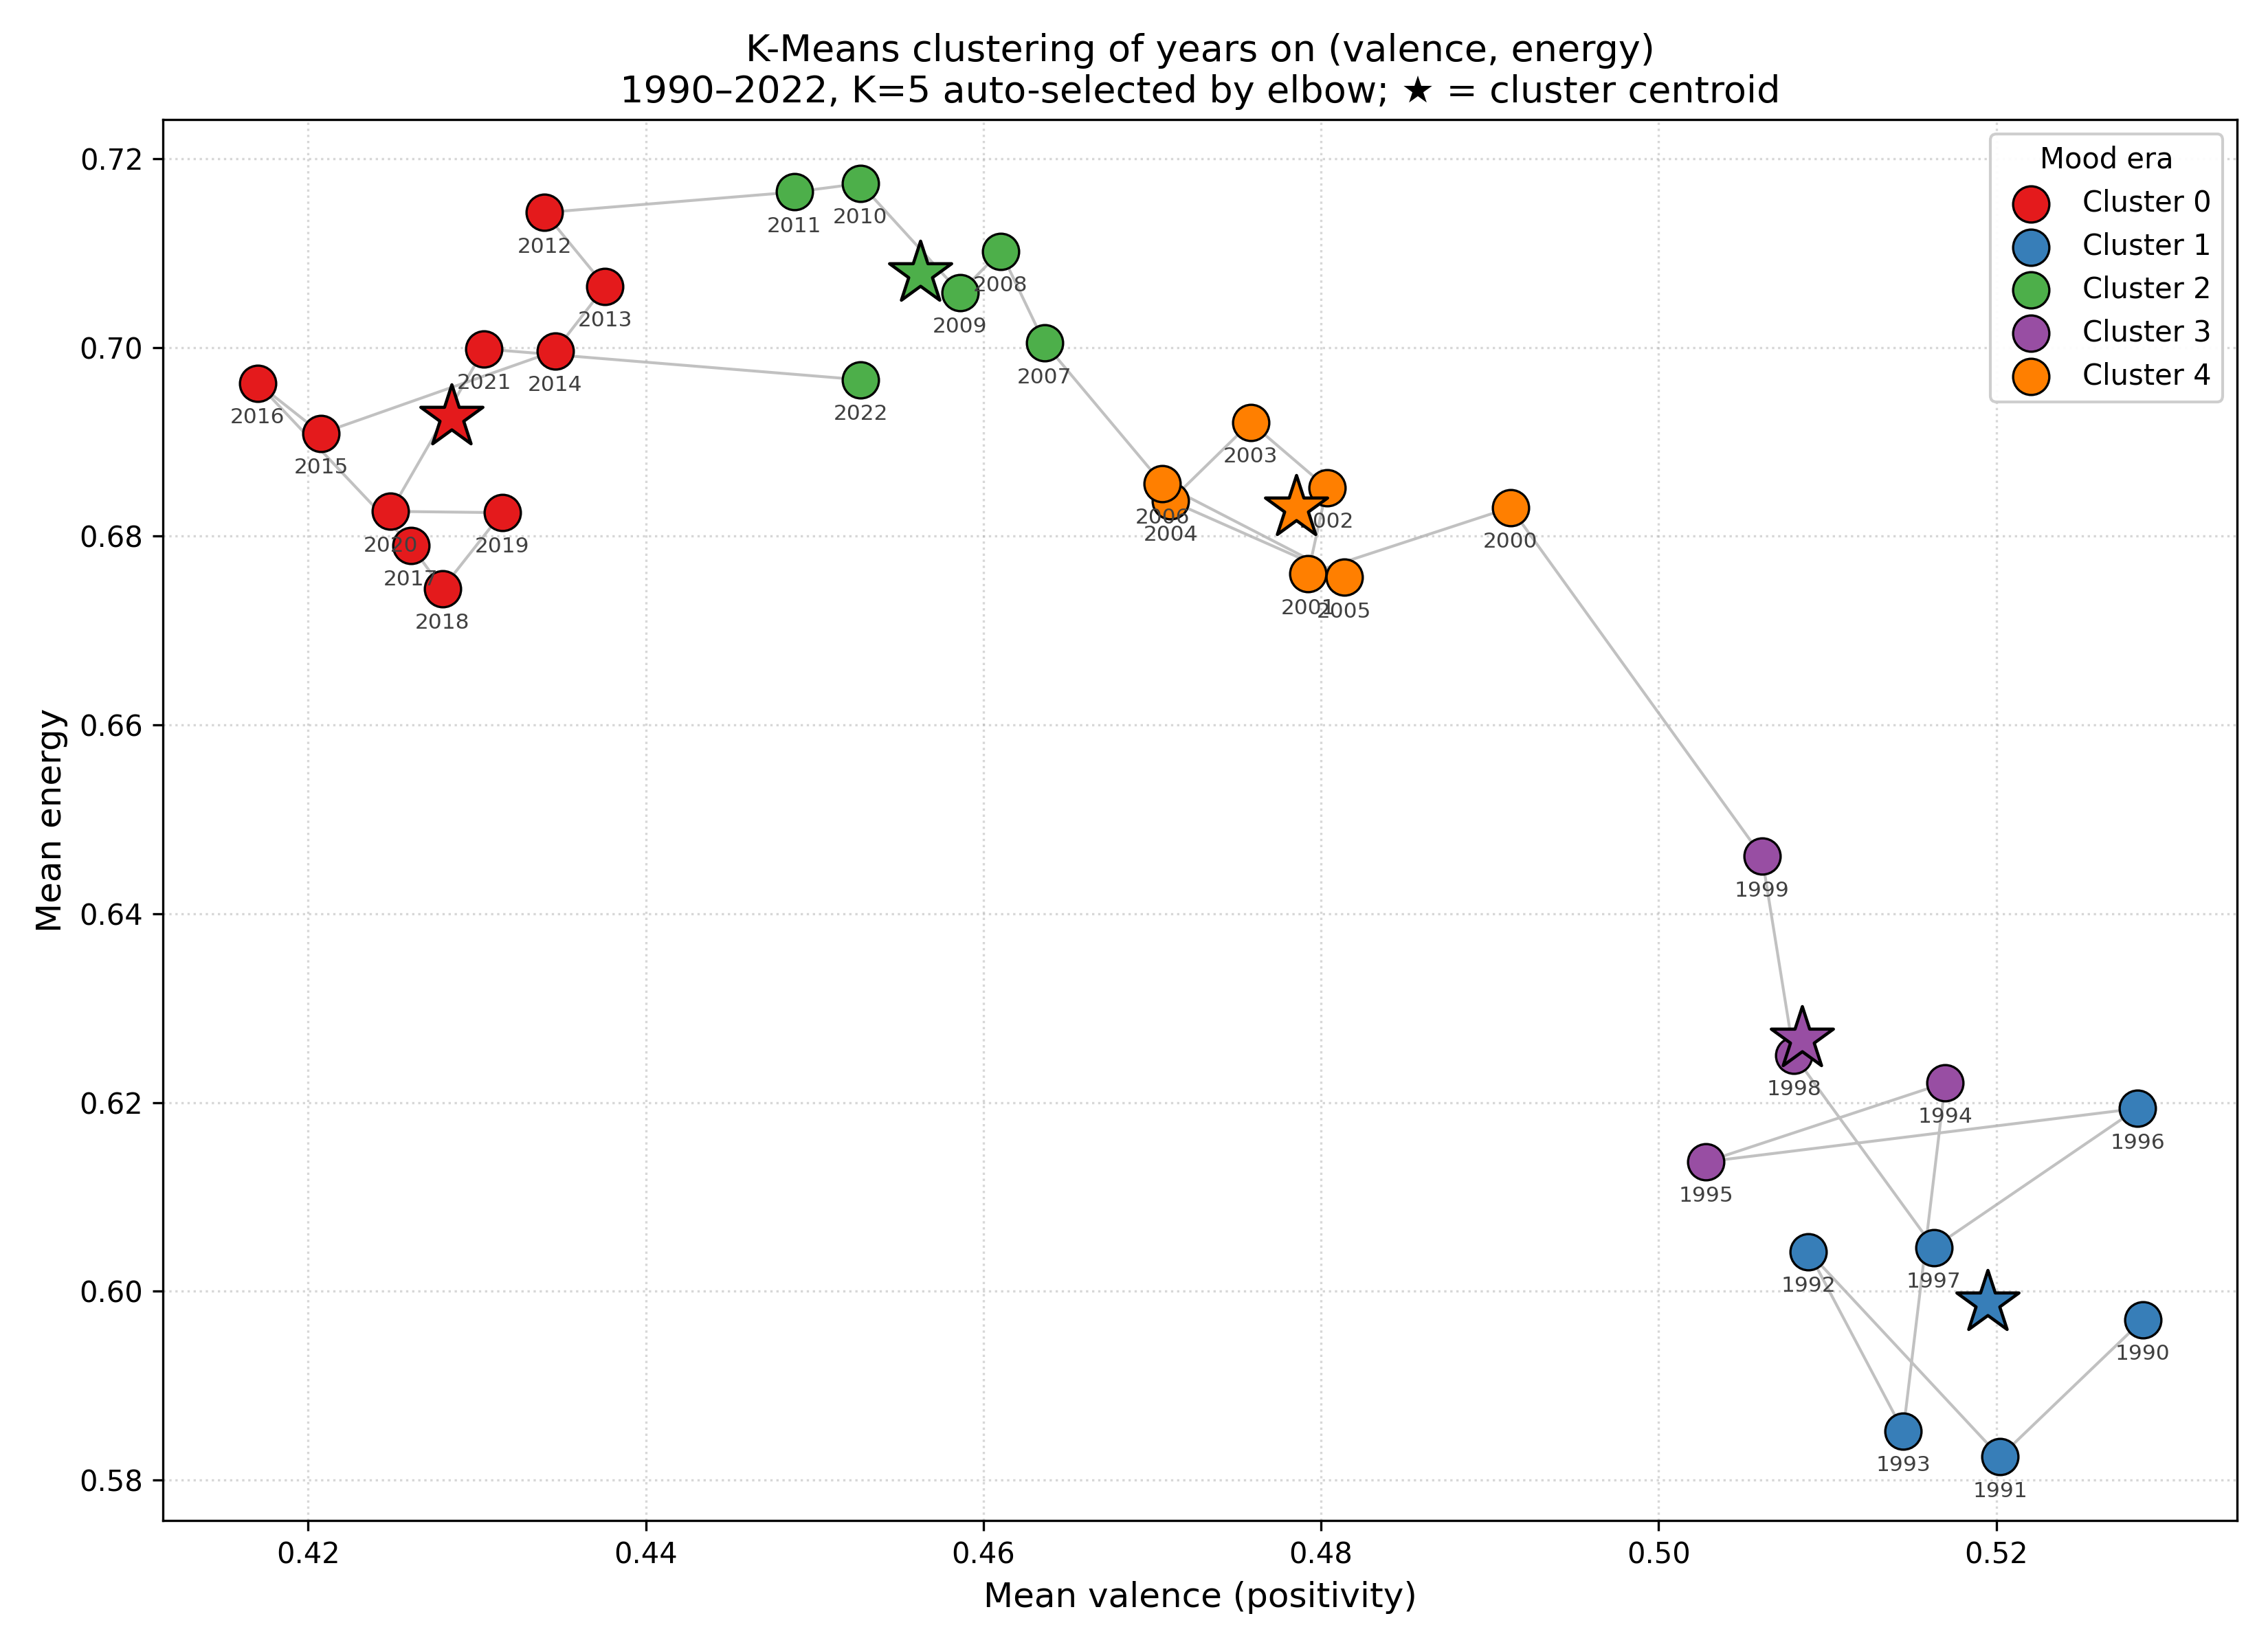
\includegraphics[width=\columnwidth]{fig1_mood_scatter.png}}
\caption{K-Means clustering of years on (valence, energy).}
\label{fig:mood}
\end{figure}

% Double-column (full width) figure -- good for the consensus raster:
\begin{figure*}[htbp]
\centerline{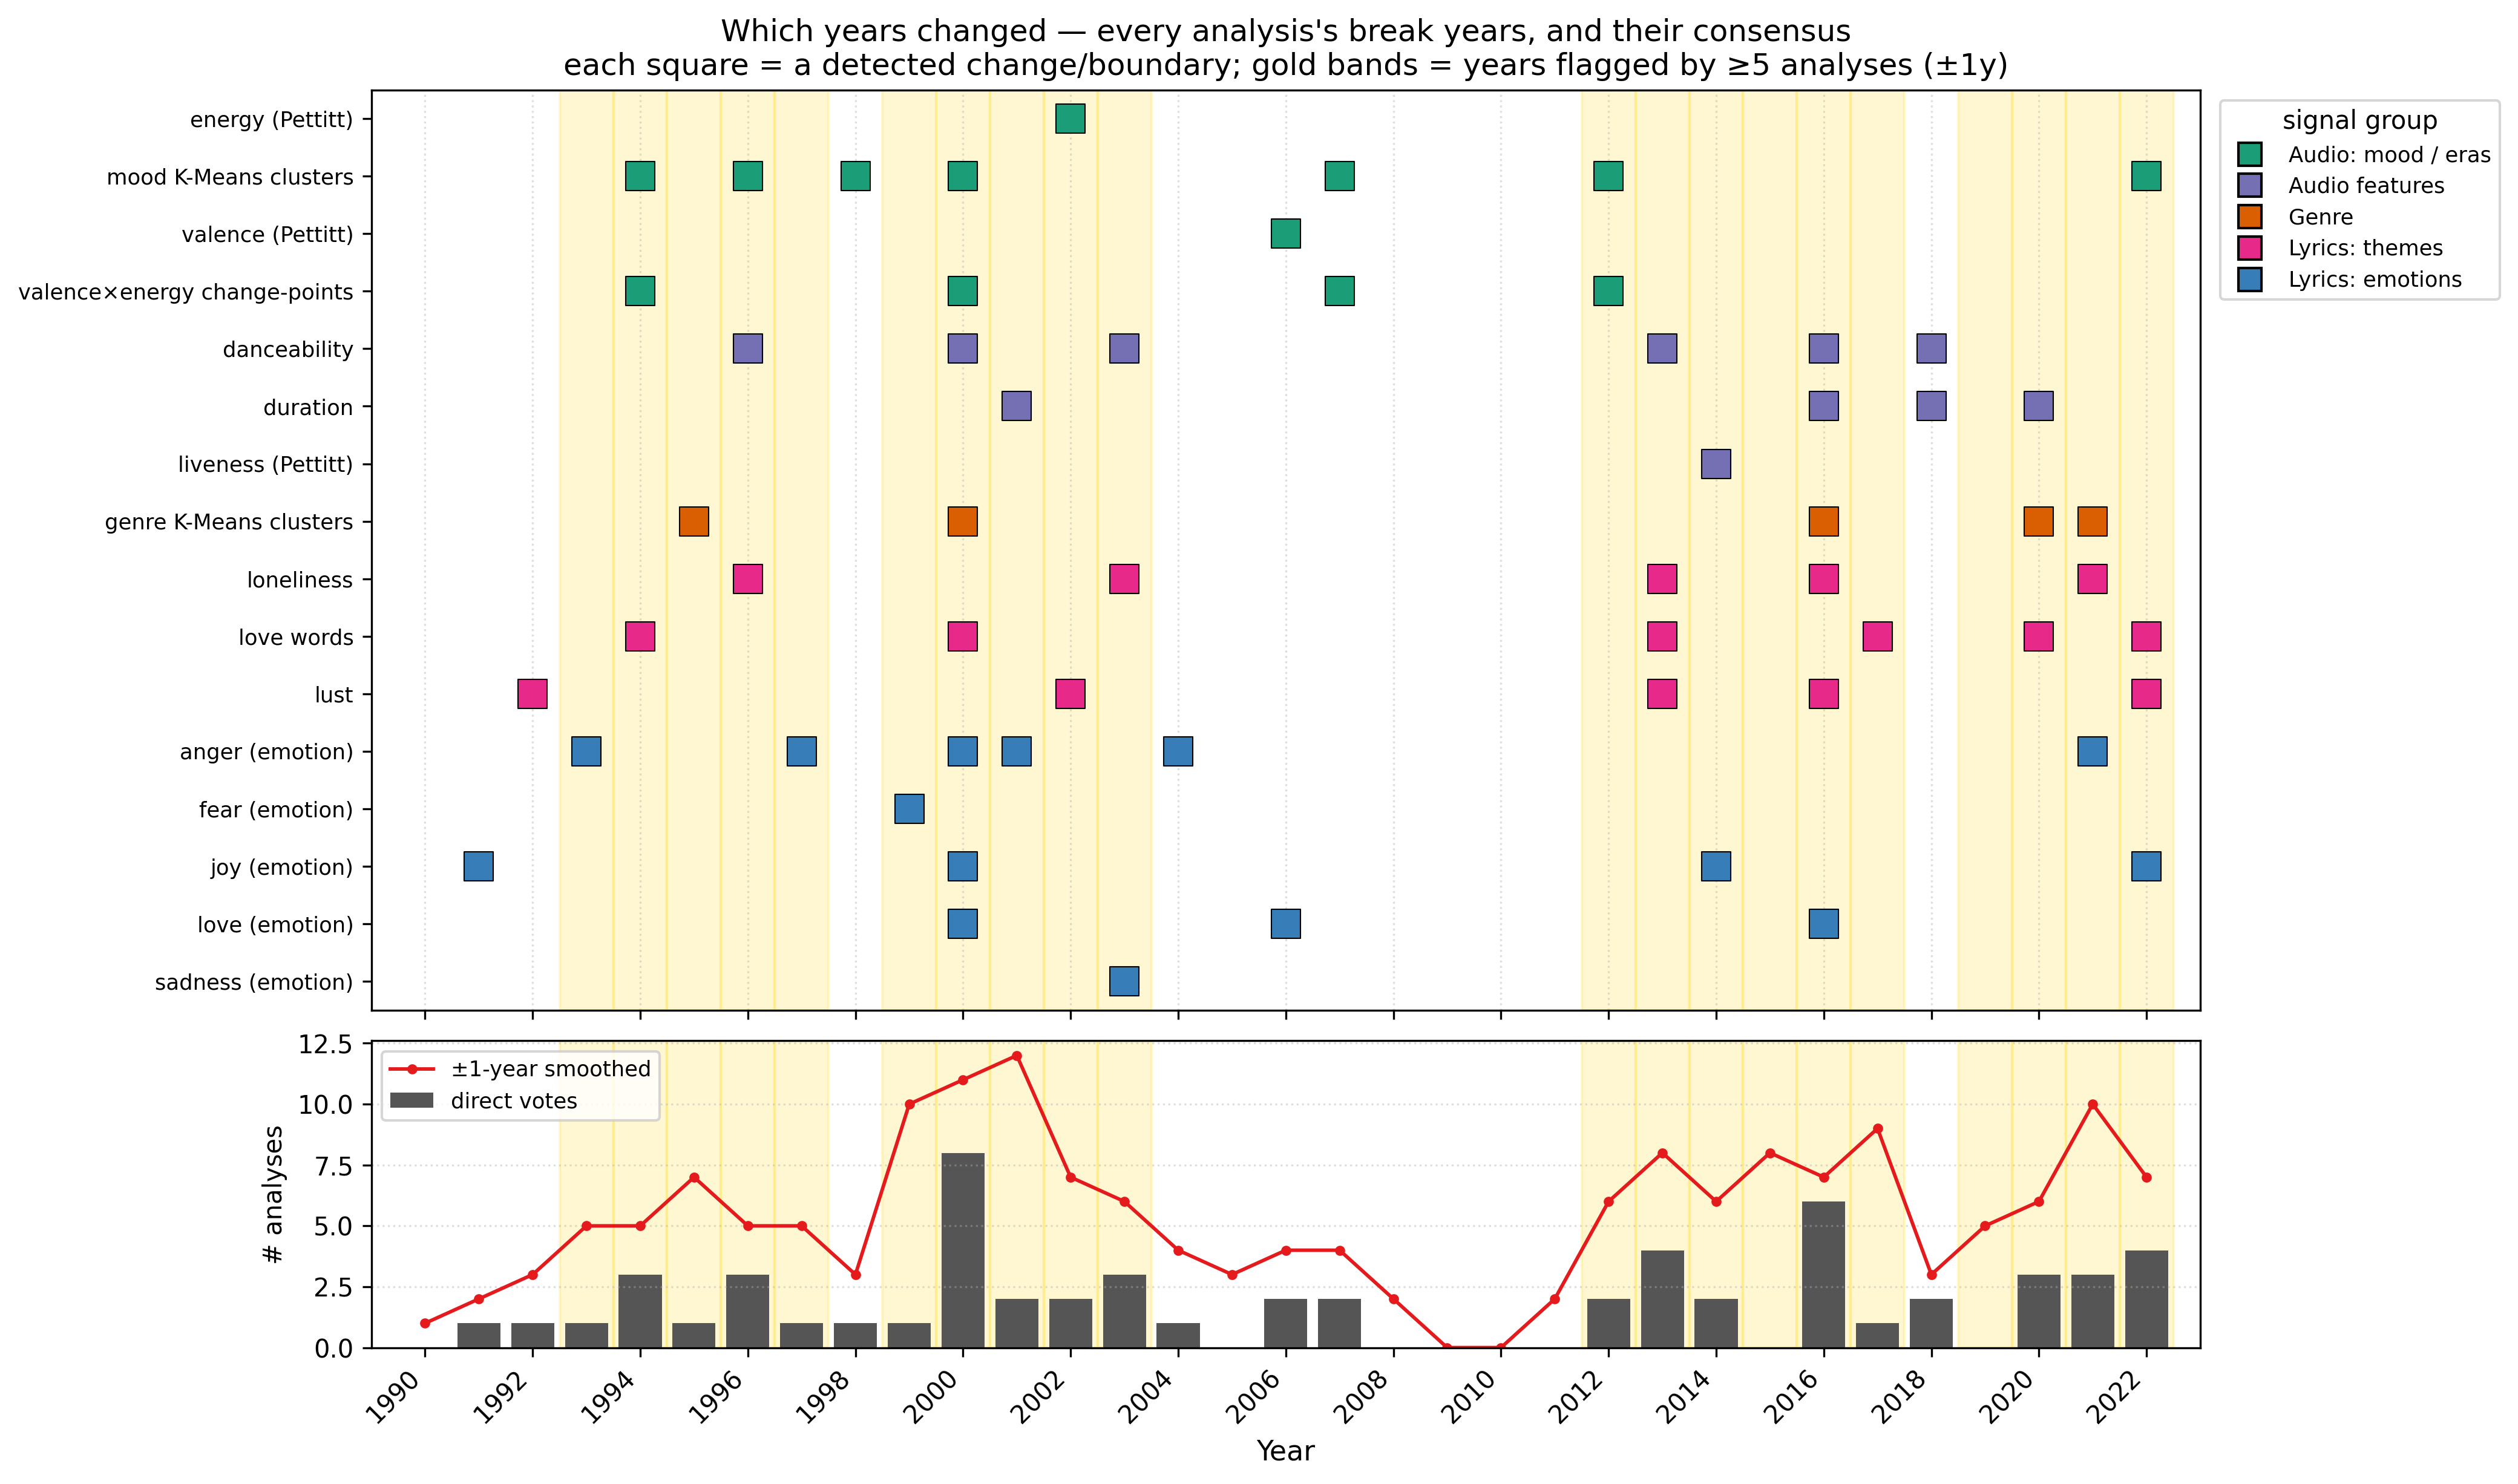
\includegraphics[width=\textwidth]{fig9_change_synthesis.png}}
\caption{Consensus of detected change years across every analysis.}
\label{fig:synthesis}
\end{figure*}

\begin{figure}[htbp]
\centerline{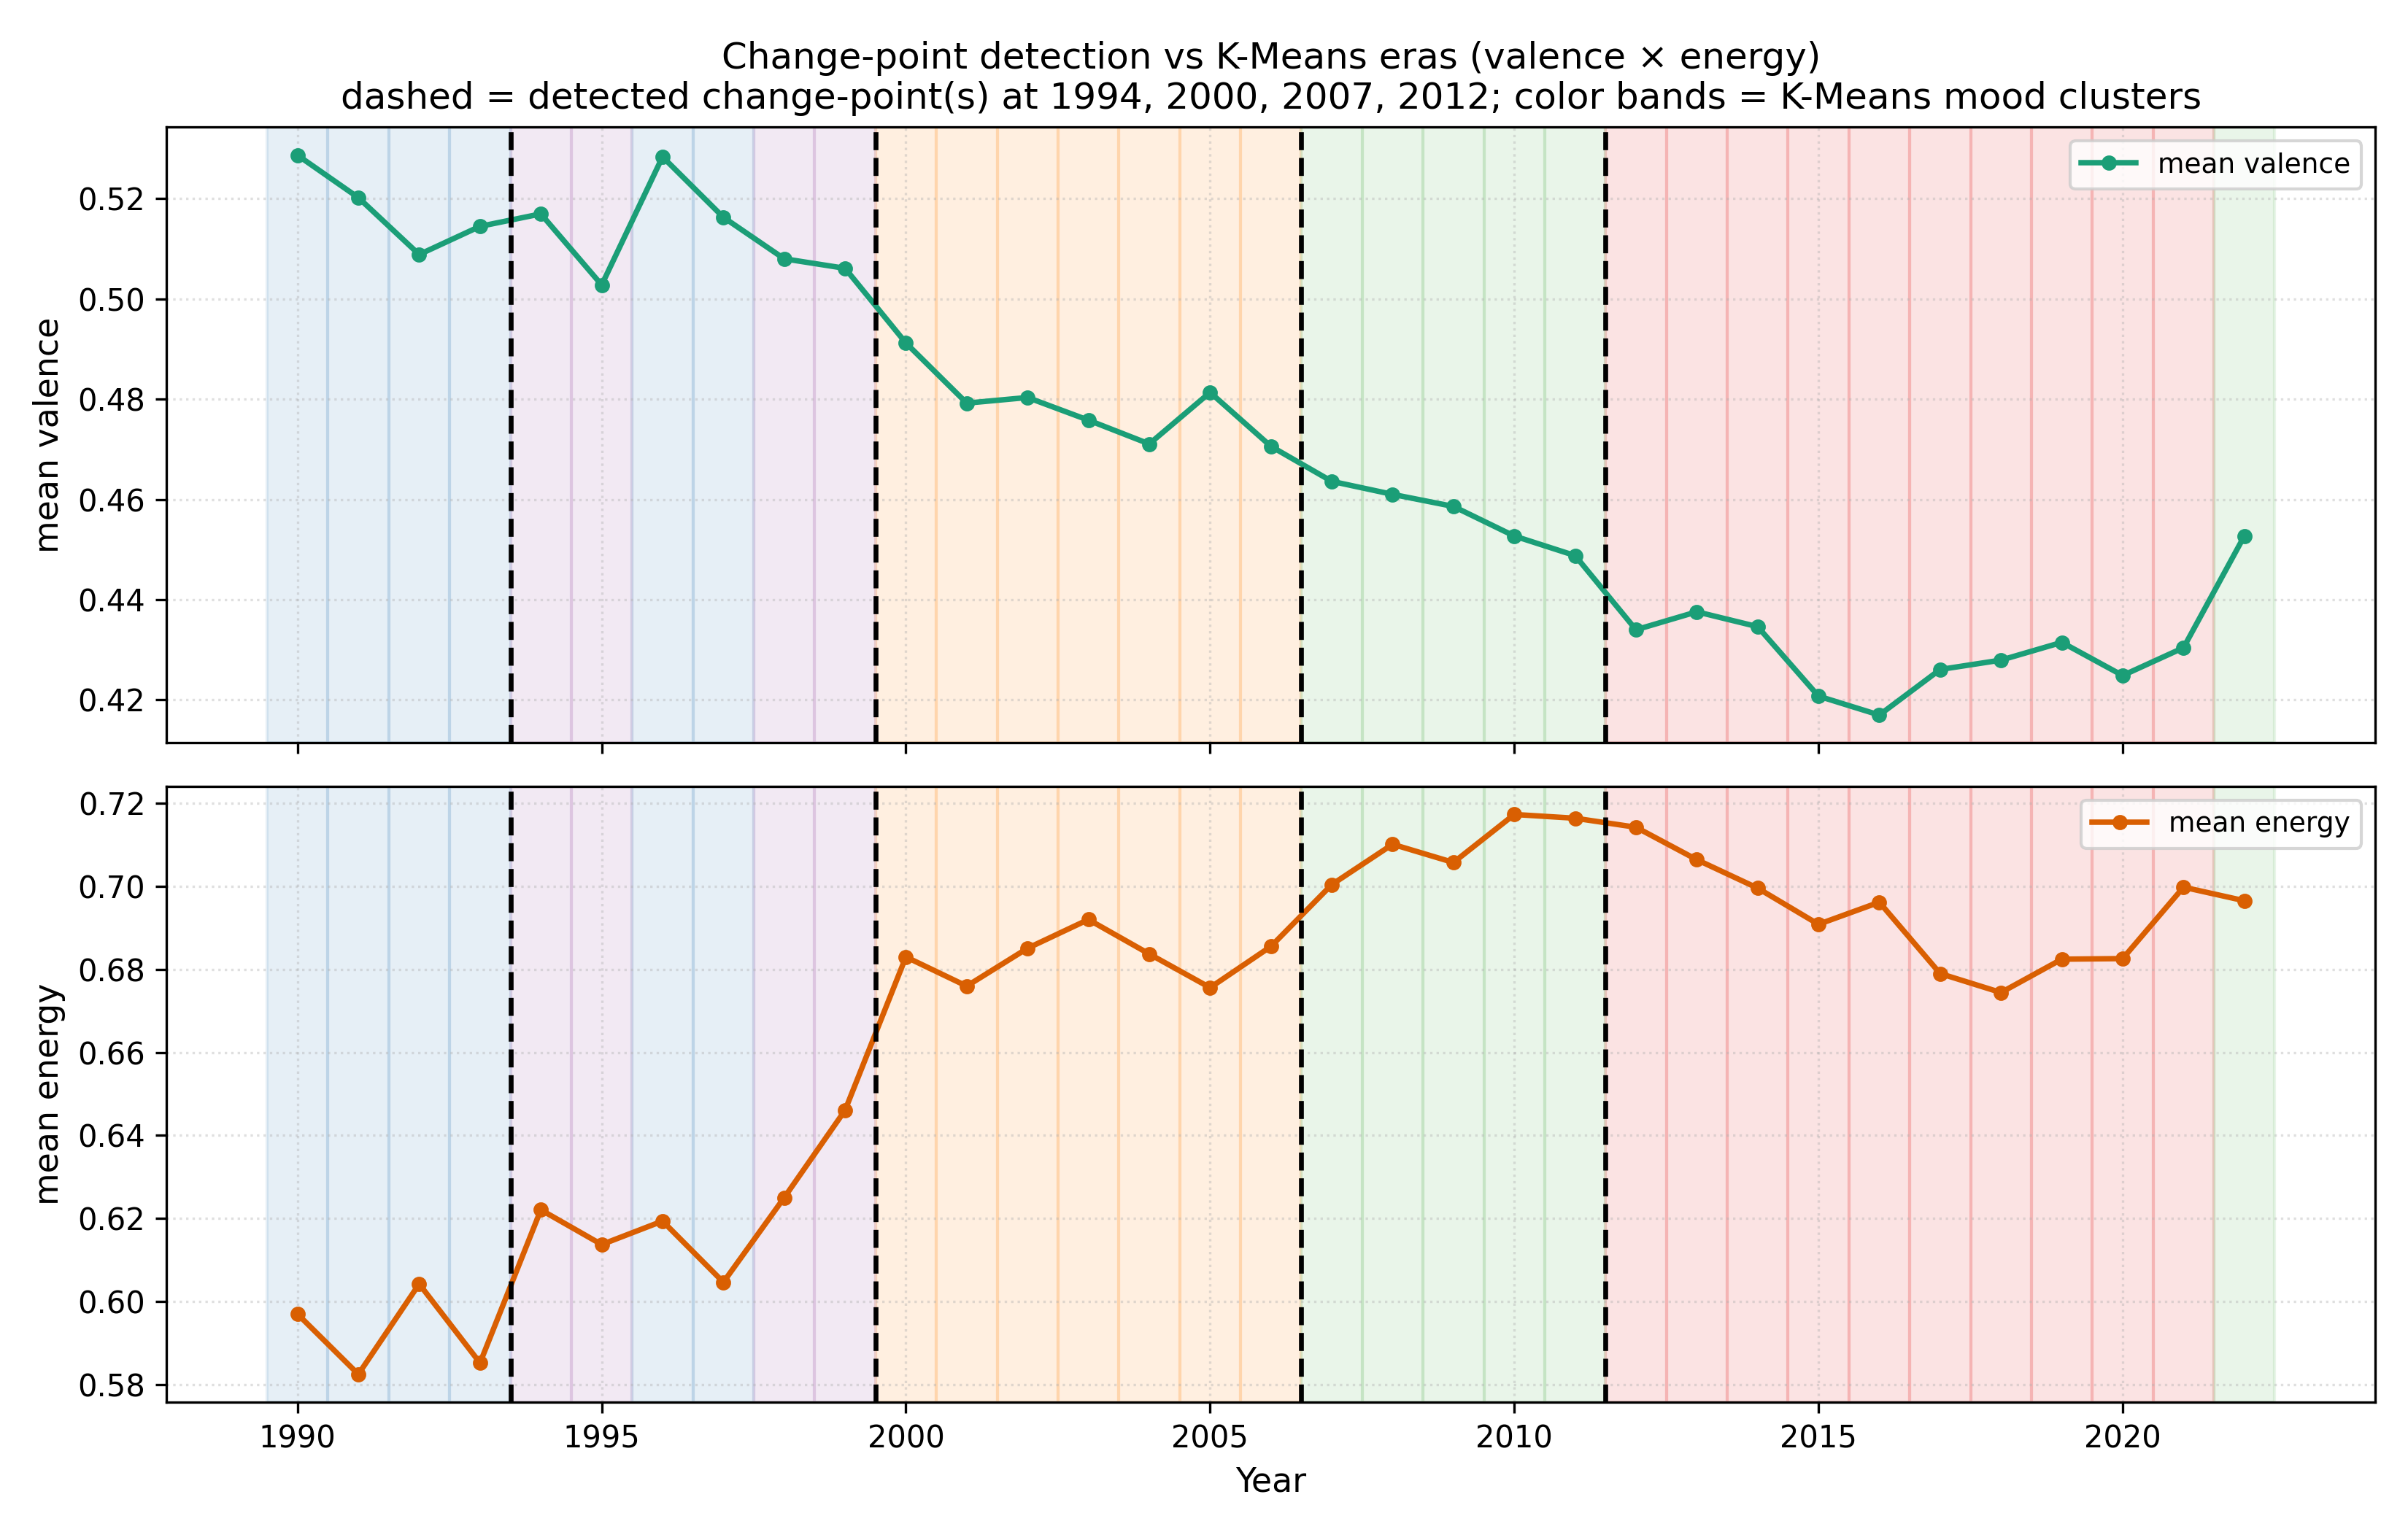
\includegraphics[width=\columnwidth]{fig6_change_points.png}}
\caption{Mean valence and energy over time with BIC-selected change-points
(dashed) and K-Means mood-cluster bands (background).}
\label{fig:changepoints}
\end{figure}

% Results table placeholder:
\begin{table}[htbp]
\caption{Mann--Kendall Trend Tests per Audio Feature, 1990--2022. Asterisks
Mark Trends Significant After Benjamini--Hochberg FDR Correction
($\alpha = 0.05$).}
\begin{center}
\begin{tabular}{|l|c|c|c|}
\hline
\textbf{Feature} & \textbf{Kendall} $\boldsymbol{\tau}$ & \textbf{$p$ (FDR)} & \textbf{Direction} \\
\hline
valence          & $-0.82$ & $2.4{\times}10^{-10}$ & decreasing$^{*}$ \\
loudness         & $+0.79$ & $6.4{\times}10^{-10}$ & increasing$^{*}$ \\
acousticness     & $-0.66$ & $2.1{\times}10^{-7}$  & decreasing$^{*}$ \\
tempo            & $+0.56$ & $1.4{\times}10^{-5}$  & increasing$^{*}$ \\
energy           & $+0.52$ & $5.4{\times}10^{-5}$  & increasing$^{*}$ \\
\hline
duration         & $-0.26$ & $0.056$ & decreasing \\
speechiness      & $+0.22$ & $0.100$ & increasing \\
instrumentalness & $-0.19$ & $0.147$ & decreasing \\
liveness         & $-0.16$ & $0.209$ & decreasing \\
danceability     & $+0.05$ & $0.698$ & increasing \\
\hline
\end{tabular}
\label{tab:trends}
\end{center}
\end{table}

\section{Discussion}

\subsection{Interpretation of the Observed Trends}
The analyses show that sonically songs became louder, faster, 
more energetic, and less acoustic over the 33-year time period, while the lyrics 
became less dominated by love and more by sadness and fear, although joy
remains as the dominant emotion in lyrics. The most interesting finding is
that the clustering of years based on valence and energy shows us that similar
years group together, and in a society where people are reporting more anxiety
and less life satisfaction, the musical analysis shows that the valence is
lowering while energy is increasing. Also, COVID-19 period and its aftermath
show some interesting results, although we cannot claim any causal relationship,
the correlation exists. Around 2020, the valence, love word count decreased
with the BERT love and happiness share while anger, sadness, and fear increasing.
According to our lexicon analysis, 2021 is a BIC change point for loneliness.

\subsection{Threats to Validity and Limitations}
Several limitations have been found. First, the corpus is a sample
from the Spotify, and real people have contributed to it by
using the Spotify's API, and the songs weren't randomly selected to
be put into the dataset provided. Second, the BERT emotion classifier model
has been trained on general text, not song lyrics, which is way more complex
with emotional expression, nuances and figurative language, which the model may
have interpreted wrongly, and has fixed weights, so fine tuning is not possible.
We have chosen 50 randomly selected songs and fed them into Claude Opus 4.8 Max
and asked it to classify the lyrics into the five emotions, and compared the results.
The LLM agent and BERT emotion model has disagreed in 32 out of 50 songs,
with ties in the BERT chunk counts broken by the model's own summed confidence
rather than an arbitrary ordering. The most disagreements arose from emotion joy,
which Claude labeled as sadness (8 times), or love (8 times). It seems like the
BERT model over-predicts joy. Third, we do not report any causal relationship 
between results and external events, we only report their correlation.

\begin{thebibliography}{00}
\bibitem{b_dataset} serkantysz, ``550K+ Spotify Songs (Audio, Lyrics, and Genres),'' Kaggle, 2024. [Online]. Available: \url{https://www.kaggle.com/datasets/serkantysz/550k-spotify-songs-audio-lyrics-and-genres}
\bibitem{b_spark} M. Zaharia \textit{et al.}, ``Apache Spark: a unified engine for big data processing,'' \textit{Commun. ACM}, vol. 59, no. 11, pp. 56--65, 2016.
\bibitem{b_sparknlp} V. Kocaman and D. Talby, ``Spark NLP: natural language understanding at scale,'' \textit{Software Impacts}, vol. 8, art. 100058, 2021.
\bibitem{b_bert} J. Devlin, M.-W. Chang, K. Lee, and K. Toutanova, ``BERT: pre-training of deep bidirectional transformers for language understanding,'' in \textit{Proc. NAACL-HLT}, 2019, pp. 4171--4186.
\bibitem{b_emotion} E. Saravia, H.-C. T. Liu, Y.-H. Huang, J. Wu, and Y.-S. Chen, ``CARER: contextualized affect representations for emotion recognition,'' in \textit{Proc. EMNLP}, 2018, pp. 3687--3697.
\bibitem{b_mk} H. B. Mann, ``Nonparametric tests against trend,'' \textit{Econometrica}, vol. 13, no. 3, pp. 245--259, 1945.
\bibitem{b_sen} P. K. Sen, ``Estimates of the regression coefficient based on Kendall's tau,'' \textit{J. Amer. Statist. Assoc.}, vol. 63, no. 324, pp. 1379--1389, 1968.
\bibitem{b_bh} Y. Benjamini and Y. Hochberg, ``Controlling the false discovery rate: a practical and powerful approach to multiple testing,'' \textit{J. Roy. Statist. Soc. B}, vol. 57, no. 1, pp. 289--300, 1995.
\bibitem{b_pettitt} A. N. Pettitt, ``A non-parametric approach to the change-point problem,'' \textit{J. Roy. Statist. Soc. C}, vol. 28, no. 2, pp. 126--135, 1979.
\bibitem{b_bic} N. R. Zhang and D. O. Siegmund, ``A modified Bayes information criterion with applications to the analysis of comparative genomic hybridization data,'' \textit{Biometrics}, vol. 63, no. 1, pp. 22--32, 2007.
\bibitem{b_kneedle} V. Satopaa, J. Albrecht, D. Irwin, and B. Raghavan, ``Finding a `kneedle' in a haystack: detecting knee points in system behavior,'' in \textit{Proc. 31st IEEE ICDCS Workshops}, 2011, pp. 166--171.
\end{thebibliography}

\end{document}
